\documentclass{article}

\usepackage[accepted]{icml2026}
\usepackage{booktabs}
\usepackage{graphicx}
\usepackage{hyperref}
\usepackage{url}

\icmltitlerunning{Reproducible Restaurant Review Sentiment Classification}

\begin{document}

\twocolumn[
\icmltitle{Reproducible Restaurant Review Sentiment Classification with
TF--IDF, Naive Bayes, and Linear SVM}

% Replace the member labels with the five names and student IDs before submission.
\begin{icmlauthorlist}
\icmlauthor{Member 1}{hku}
\icmlauthor{Member 2}{hku}
\icmlauthor{Member 3}{hku}
\icmlauthor{Member 4}{hku}
\icmlauthor{Member 5}{hku}
\end{icmlauthorlist}

\icmlaffiliation{hku}{STAT8017 Data Mining Techniques, The University of Hong Kong}
\icmlcorrespondingauthor{Member 1}{replace-with-group-email@example.com}

\vskip 0.3in
]

\printAffiliationsAndNotice{}

\begin{abstract}
We study binary sentiment classification for a fixed public snapshot of 1,000
restaurant-review snippets. After removing four same-label duplicate rows, we
create one stratified 796/200 training/test split and compare word-unigram and
unigram--bigram TF--IDF representations without fitting vocabulary or inverse
document frequencies on validation or test text. Training-fold validation
selects word unigrams, Linear SVM with $C=0.1$, and Multinomial Naive Bayes with
$\alpha=0.5$. On the held-out test partition, Naive Bayes obtains F1 0.742 and
ROC--AUC 0.837, while Linear SVM obtains F1 0.720 and ROC--AUC 0.806. We report
data quality checks, model interpretation, and descriptive error categories,
and provide a fully reproducible code and notebook workflow.
\end{abstract}

\section{Introduction}

Short restaurant reviews express sentiment through sparse lexical cues,
negation, and context. This project asks whether a linear support vector
machine or Multinomial Naive Bayes is more effective for a small labelled text
dataset, whether adjacent bigrams improve over word unigrams, and which error
patterns remain after model selection. We use TF--IDF because it provides a
transparent sparse representation that is compatible with both classifiers.

Our experimental design separates representation selection and hyperparameter
tuning from final evaluation. Every cross-validation fold refits the complete
TF--IDF and classifier pipeline, while the fixed test partition is excluded
from feature and parameter selection. The repository records data hashes,
random seeds, dependency versions, aggregate predictions, and an independent
Member 1 reproduction manifest so that every reported number can be traced to
code.

\section{Dataset and Exploratory Data Analysis}
\label{sec:data-eda}

\paragraph{Dataset and data quality.}
We analysed 1,000 English restaurant-review snippets from the public
\texttt{Restaurant\_Reviews.tsv} snapshot
\citep{rajagopal-restaurant-reviews}. The file contains review text
(\texttt{Review}) and a binary sentiment label (\texttt{Liked}, with 0
for negative and 1 for positive), with 500 observations per class.
A row-wise comparison with the UCI Yelp subset \citep{kotzias-sentiment}
found 995 matching text--label pairs after trimming whitespace.
We use the TSV snapshot for all counts below.

We checked for missing fields, blank reviews, unsupported labels,
duplicate text and unusual characters. We applied Unicode NFC
normalization, collapsed whitespace and kept punctuation, accents and
negation. The file contained four reviews with non-ASCII characters,
zero missing or blank fields, and zero flagged control or replacement
characters. Four redundant same-label records were removed before
splitting, and there were zero identical texts with conflicting labels.
The resulting corpus contained 996 distinct reviews, with 497 negative
and 499 positive.

\paragraph{Data partition.}
We used a single stratified 80/20 split with random seed 8017
(Table~\ref{tab:data-eda-split}). The test set contained 100 reviews
per class, and the two partitions shared zero exact review texts after
normalization. Subsequent feature fitting and model selection use the
training partition. The test partition is reserved for final evaluation.

\begin{table}[t]
  \caption{Class counts after deduplication and stratified splitting.}
  \label{tab:data-eda-split}
  \centering
  \begin{tabular}{lrrr}
    \hline
    Partition & Negative & Positive & Total \\
    \hline
    Cleaned & 497 & 499 & 996 \\
    Train & 397 & 399 & 796 \\
    Test & 100 & 100 & 200 \\
    \hline
  \end{tabular}
\end{table}

\paragraph{Review length and vocabulary.}
Negative reviews had a median length of 10 words (interquartile range
6--16), compared with 9 words (6--14) for positive reviews
(Figure~\ref{fig:data-eda-lengths}). The overlapping distributions
suggest that length alone offers limited separation. In the training
set, \emph{not} appeared in 81 of 397 negative reviews (20.4\%).
\emph{Good} appeared in 59 of 399 positive reviews (14.8\%) and 18 of
397 negative reviews (4.5\%). This overlap motivates evaluating
bigrams that can represent local context. We counted each word once per
review for these frequencies and retained negation during stop-word
filtering. The source file has no restaurant or reviewer identifiers,
so the split measures generalization at the review level.

\begin{figure}[t]
  \centering
  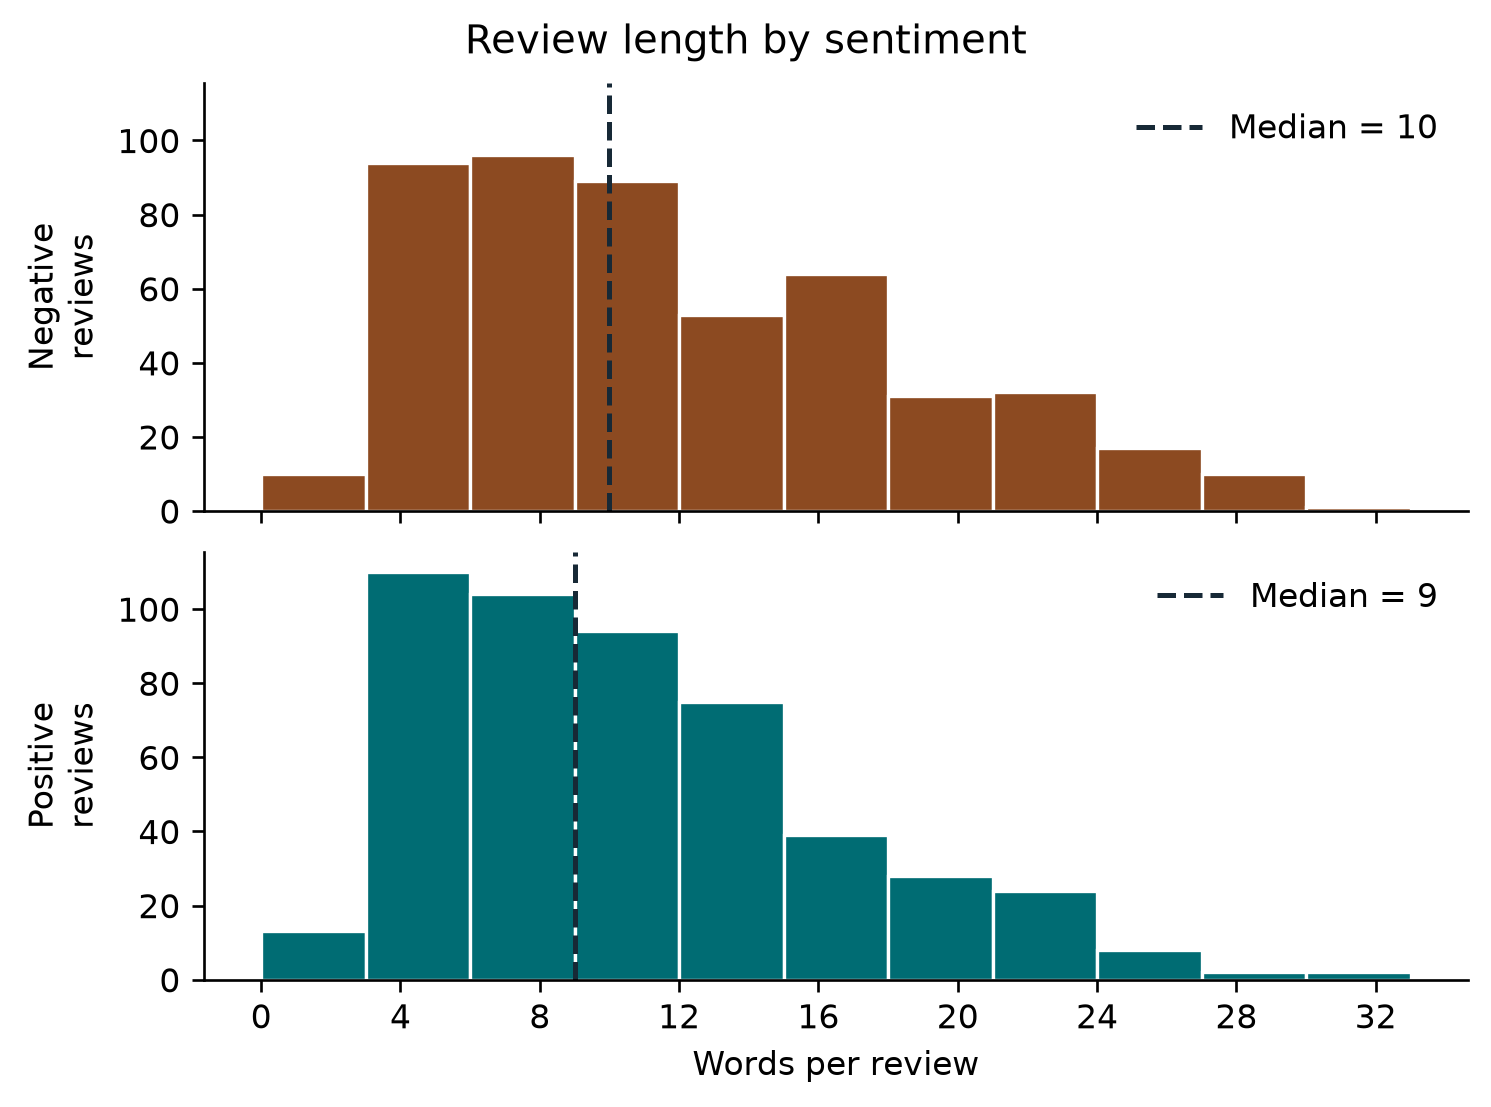
\includegraphics[width=\columnwidth]{../results/figures/eda_review_lengths.png}
  \caption{Word counts in the cleaned corpus by sentiment. The panels
  share histogram bins and axes. Dashed lines mark the class medians.}
  \label{fig:data-eda-lengths}
\end{figure}

\section{Text Preprocessing and Feature Representation}
\label{sec:text-features}

\paragraph{Representation.}
We used the fixed 796-review training partition and reserved the
200-review test partition for subsequent final evaluation.
After the shared data cleaning, we lowercased text and applied Unicode
accent stripping. The word tokenizer retained tokens of at least two
word characters. We did not remove stop words or apply stemming or
lemmatization, retaining explicit negation words such as \emph{not},
\emph{no}, and \emph{never}. The default tokenizer nevertheless splits
contractions and drops single-character fragments; this does not
preserve all contracted negation. Punctuation intensity and long-range
word order are not represented.

We compared word unigrams with word unigrams plus adjacent bigrams using
scikit-learn's TF--IDF implementation \citep{pedregosa2011scikit,manning2008ir}.
Term frequency was scaled as $1+\ln(c)$ for positive count $c$.
Smoothed inverse document frequency was
$\ln((1+n)/(1+\mathrm{df}))+1$, followed by document-wise L2 normalization.
We set \texttt{min\_df=1}, \texttt{max\_df=1.0}, and imposed no vocabulary
cap. The resulting nonnegative features are compatible with both
Multinomial Naive Bayes and Linear SVM.

\paragraph{Training-only comparison.}
We used identical five-fold stratified training splits with shuffling
and random seed 8017. A fresh vectorizer and classifier were fitted
inside every fold; validation texts did not determine vocabulary or IDF.
Linear SVM with fixed $C=1$ was the feature-selection probe, and
Multinomial Naive Bayes with fixed $\alpha=1$ was a sensitivity check.
We selected the representation by mean positive-class validation F1
under the SVM probe, preferring unigrams in an exact tie. This experiment
does not replace later classifier tuning or final test evaluation.

\begin{table}[t]
  \caption{Training-only five-fold feature comparison. Values are mean
  positive-class F1 and sample standard deviation across folds, not
  confidence intervals. No test-set performance is reported.}
  \label{tab:tfidf-ablation}
  \centering
  \resizebox{\columnwidth}{!}{%
  \begin{tabular}{llr}
    \hline
    Features & Probe & F1 mean $\pm$ SD \\
    \hline
    Unigram & Linear SVM & $0.8016 \pm 0.0282$ \\
    Unigram + bigram & Linear SVM & $0.7998 \pm 0.0388$ \\
    Unigram & Multinomial NB & $0.7962 \pm 0.0484$ \\
    Unigram + bigram & Multinomial NB & $0.7845 \pm 0.0394$ \\
    \hline
  \end{tabular}
  }
\end{table}

\paragraph{Feature summary and handoff.}
Unigrams yielded a mean SVM validation F1 of 0.8016, compared with
0.7998 for unigrams plus bigrams (Table~\ref{tab:tfidf-ablation}).
The difference of approximately 0.0018 was small relative to fold
variability and does not establish a significant or general advantage.
Although bigrams slightly increased mean SVM accuracy
(0.8041 versus 0.8015) and ROC-AUC (0.8972 versus 0.8953),
they did not improve the prespecified F1 criterion.
We therefore recommend unigrams as the shared default.

Fitting on the full training partition produced 1,781 unigram features
and 7,345 unigram--bigram features, a 4.12-fold increase in dimension.
The training matrices contained 7,836 and 15,269 nonzero entries,
respectively, with densities of 0.553\% and 0.261\%.
All training and transformed test rows had at least one nonzero feature.
The larger phrase vocabulary may be difficult to estimate reliably
from this small corpus. We exported sparse matrices, ordered row IDs,
vocabularies, fitted vectorizers, and parameter metadata for subsequent
members. Test texts were transformed only after fitting on training
texts. Classifier cross-validation must still refit the full pipeline
within each fold rather than reuse these full-training fitted matrices.


\section{Methods and Experimental Setup}
\label{sec:methods}

All experiments use the same word-unigram TF--IDF settings selected in
Section~\ref{sec:text-features}. Hyperparameters are selected by mean
positive-class F1 under five-fold stratified cross-validation with shuffling
and random seed 8017. Accuracy, precision, recall, F1, and ROC--AUC are retained
for diagnosis. The majority-class classifier is included as a minimum
baseline.

\subsection{Linear Support Vector Machine}
\label{sec:linear-svm}

The principal classifier was a linear support vector machine (SVM), which is well suited to high-dimensional sparse text representations. A linear decision function $f(\mathbf{x})=\mathbf{w}^{\top}\mathbf{x}+b$ was estimated by minimizing regularized hinge loss; the sign of $f(\mathbf{x})$ determined the predicted sentiment. The regularization parameter $C$ controls the trade-off between a wider margin and penalties for training errors: smaller values impose stronger regularization, whereas larger values fit the training observations more aggressively \citep{cortes1995support}. We used scikit-learn's \texttt{LinearSVC} implementation \citep{pedregosa2011scikit}.

All SVM experiments used the fixed 796-review training partition and the unigram TF--IDF representation selected in the preceding feature experiment. To prevent information leakage, the vectorizer was fitted again inside every validation fold as part of a single pipeline. We compared $C\in\{0.1,1,10\}$ using five-fold stratified cross-validation with shuffled folds and random seed 8017. The selection criterion was mean positive-class F1; accuracy, precision, recall, and ROC--AUC were retained as secondary diagnostics. The held-out 200-review test partition was not inspected during this selection.

\begin{table}[t]
\centering
\caption{Training-only five-fold cross-validation for Linear SVM. Values are fold means; the selected setting is bold.}
\label{tab:svm-cv}
\small
\resizebox{\columnwidth}{!}{%
\begin{tabular}{rrrrrr}
\toprule
$C$ & Accuracy & Precision & Recall & F1 & ROC--AUC \\
\midrule
\textbf{0.1} & \textbf{0.8104} & \textbf{0.8224} & 0.7922 & \textbf{0.8060} & 0.8850 \\
1.0 & 0.8015 & 0.8054 & 0.7996 & 0.8016 & \textbf{0.8953} \\
10.0 & 0.8015 & 0.8051 & \textbf{0.8021} & 0.8022 & 0.8915 \\
\bottomrule
\end{tabular}
}
\end{table}

The mean F1 values were close, but $C=0.1$ achieved the highest validation F1 (0.8060) and accuracy (0.8104), so it was locked before test evaluation. After refitting the complete pipeline on all training reviews, the model obtained test accuracy 0.7400, precision 0.7791, recall 0.6700, F1 0.7204, and ROC--AUC 0.8061. The precision--recall imbalance indicates that the locked classifier was relatively conservative in assigning positive sentiment. These test results should be reported alongside the Naive Bayes and majority baselines in the unified evaluation section rather than interpreted as an isolated model comparison.

The fitted linear coefficients also provide a direct interpretation of influential features. The strongest negative weights included \textit{not}, \textit{wasn't}, \textit{bad}, \textit{terrible}, and \textit{worst}; the strongest positive weights included \textit{great}, \textit{good}, \textit{delicious}, \textit{fantastic}, and \textit{amazing}. These coefficients describe associations in this corpus rather than causal effects, and isolated tokens can be misleading when sentiment depends on composition or context.

\section{Naive Bayes Methodology}
\label{sec:nb-method}

\paragraph{Model.}
We trained a Multinomial Naive Bayes classifier \citep{manning2008ir} on the
same word-unigram TF--IDF representation used by the Linear SVM and the
majority-class baseline \citep{pedregosa2011scikit}. For a document with
nonnegative, L2-normalized features $x$, the decision rule is
$\hat{c} = \arg\max_{c} [\log P(c) + \sum_j x_j \log P(w_j \mid c)]$.
Additive (Laplace) smoothing with parameter $\alpha$ prevents zero term
probabilities. We did not add stemming, stop-word removal, or any rescaling
beyond the shared pipeline; the fitted vectorizer therefore remains identical
across classifiers.

\paragraph{Smoothing selection on training folds only.}
We compared $\alpha \in \{0.1, 0.5, 1.0, 2.0\}$ with five-fold stratified
cross-validation on the 796 training reviews, using shuffling and random seed
8017. A fresh TF--IDF--NB pipeline was fitted inside every fold, so validation
terms and IDF weights never leaked into feature construction. The prespecified
selection criterion was mean positive-class F1, with ties preferring the
smaller $\alpha$; the 200 reviews in the test partition were not used.

\begin{table}[t]
  \caption{Training-fold Multinomial NB smoothing comparison (796 reviews,
  five stratified folds, seed 8017). Values are means with population standard
  deviations; these are validation results, not test-set performance.}
  \label{tab:nb-alpha}
  \centering
  \begin{tabular}{rrrr}
    \hline
    $\alpha$ & Accuracy & F1 & ROC-AUC \\
    \hline
    0.1 & $0.7864 \pm 0.0325$ & $0.7849 \pm 0.0317$ & $0.8735 \pm 0.0246$ \\
    \textbf{0.5} & $\mathbf{0.8065 \pm 0.0384}$ & $\mathbf{0.8052 \pm 0.0390}$ & $\mathbf{0.8818 \pm 0.0278}$ \\
    1.0 & $0.7965 \pm 0.0398$ & $0.7962 \pm 0.0433$ & $0.8802 \pm 0.0304$ \\
    2.0 & $0.7877 \pm 0.0419$ & $0.7905 \pm 0.0461$ & $0.8787 \pm 0.0329$ \\
    \hline
  \end{tabular}
\end{table}

Table~\ref{tab:nb-alpha} shows a broad optimum near $\alpha=0.5$, which was
selected for the final fit. The spread across $\alpha$ values is small relative
to fold-to-fold variation, so this is a practical choice rather than evidence
that the other smoothing values are inferior. The value $\alpha=1$ gave a mean
F1 of 0.7962, consistent with the independent feature probe of Member 3.

\section{Results}
\label{sec:results}

\paragraph{Final comparison.}
All models were fitted on the same 796 training reviews and evaluated once on
the same untouched 200-review test partition (100 reviews per class). NB used
the training-fold-selected $\alpha=0.5$; Linear SVM used $C=0.1$, selected by
Member 4 through five-fold training-only cross-validation. The test set was not
used to choose either parameter.

\begin{table}[t]
  \caption{Final test-set comparison on 200 reviews. ``Dummy'' predicts the
  majority training class. F1 and precision refer to the positive (Liked=1)
  class. NB scores are predicted probabilities; SVM scores are decision
  function values; both are rank-valid for ROC-AUC.}
  \label{tab:final-comparison}
  \centering
  \begin{tabular}{lrrrrr}
    \hline
    Model & Accuracy & Precision & Recall & F1 & ROC-AUC \\
    \hline
    Dummy (majority) & 0.500 & 0.500 & 1.000 & 0.667 & 0.500 \\
    Multinomial NB ($\alpha=0.5$) & 0.750 & 0.766 & 0.720 & \textbf{0.742} & 0.837 \\
    Linear SVM ($C=0.1$) & 0.740 & \textbf{0.779} & 0.670 & 0.720 & 0.806 \\
    \hline
  \end{tabular}
\end{table}

Both learned classifiers clearly outperformed the majority-class baseline.
NB obtained higher accuracy, recall, positive-class F1 and ROC-AUC, while SVM
had higher precision. On the confusion matrices,
NB produced 78 true negatives, 22 false positives, 28 false negatives and 72
true positives; SVM produced 81, 19, 33 and 67 in the same order. Thus NB
recalled more positive reviews, whereas SVM made fewer false-positive errors.
With 200 test reviews, a one-review change can shift accuracy by 0.005, and no
significance test supports a general ranking beyond this fixed sample.

\begin{figure}[t]
  \centering
  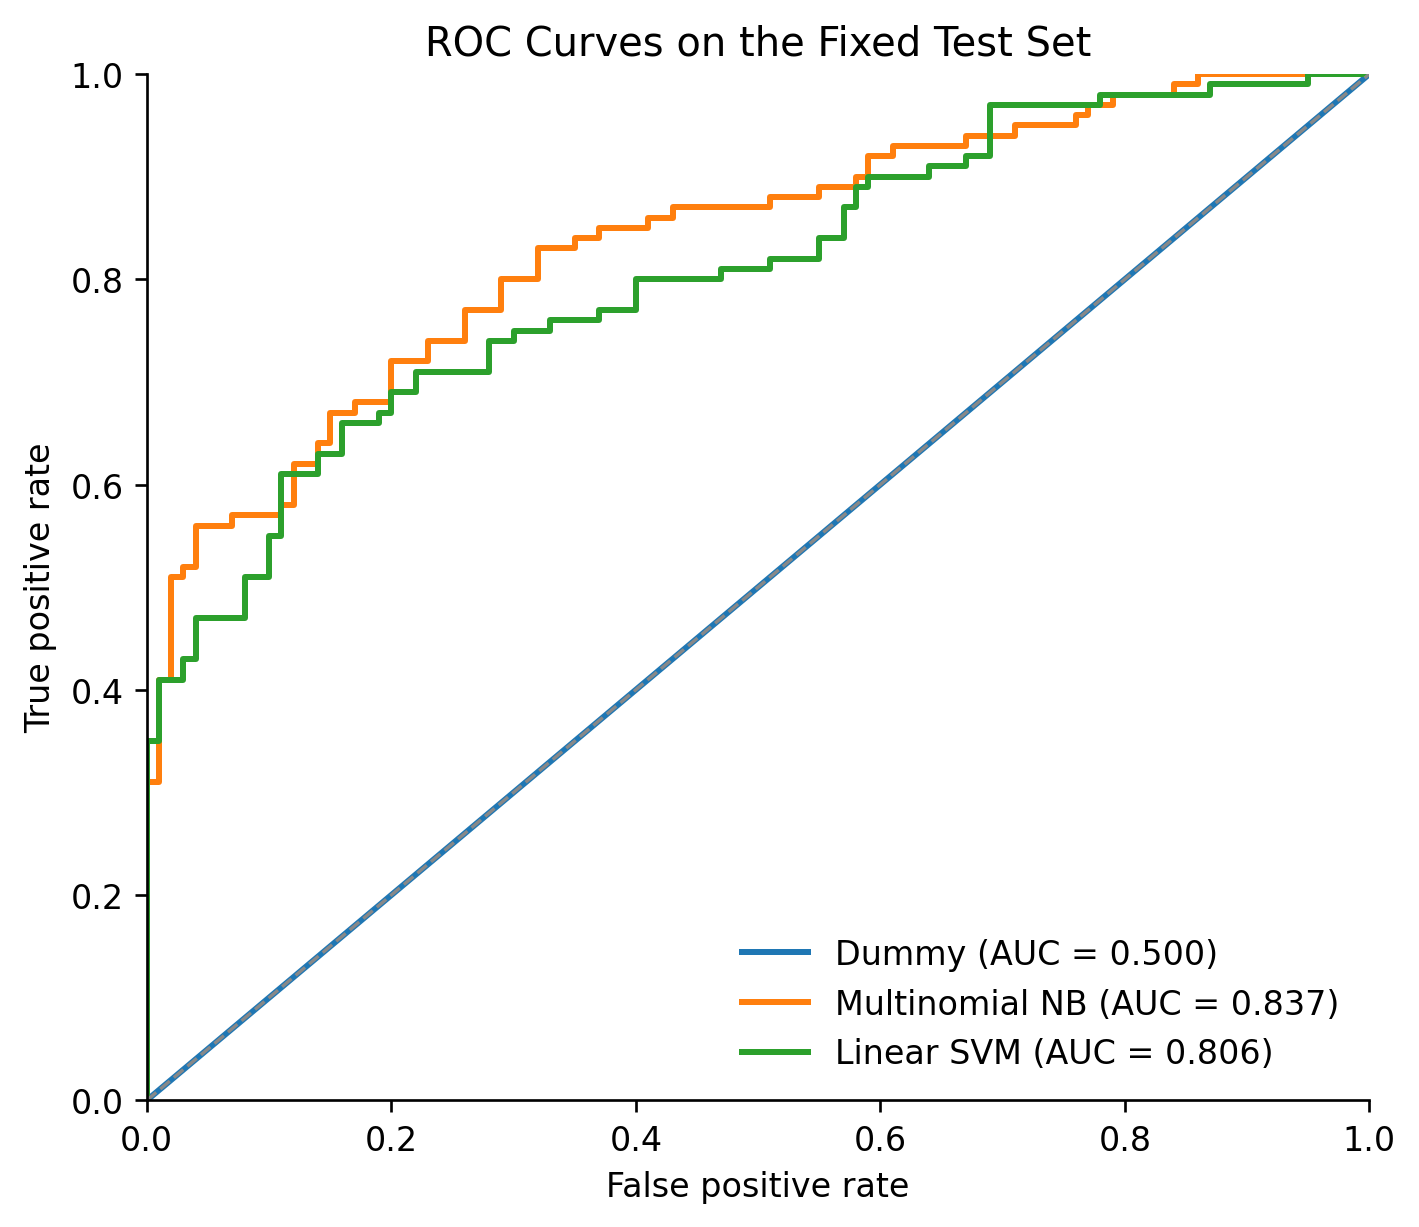
\includegraphics[width=\columnwidth]{../results/figures/final_roc_curves.png}
  \caption{ROC curves of all three models on the fixed test partition. The
  diagonal is the random-classification baseline. The legend reports the
  area under each curve.}
  \label{fig:final-roc}
\end{figure}

As shown in Figure~\ref{fig:final-roc}, NB achieved stronger ranking quality
than the locked SVM on this test set (AUC 0.837 versus 0.806). The curves still
cross at some operating points, so deployment choices should consider the
desired precision--recall trade-off rather than AUC alone.

\paragraph{Interpretation of learned weights.}
The strongest positive NB log-odds terms include \emph{great},
\emph{delicious}, \emph{fantastic} and \emph{awesome}; the strongest negative
terms include \emph{terrible}, \emph{bad}, \emph{slow} and the truncated token
\emph{wasn}. The SVM assigns large negative weights to \emph{not}, \emph{wasn}
and \emph{don}. These weights reflect corpus frequency and the tokenizer's
treatment of contractions: \emph{isn't} becomes \emph{isn} plus a discarded
single-character fragment, so the model cannot reliably interpret contracted
negation. High weights are explanatory cues, not causal evidence about what
makes a review positive or negative.

\section{Error Analysis}
\label{sec:error-analysis}

We inspected every test review that was misclassified and assigned one
descriptive category by a fixed priority: mixed positive and negative cue
words, negation or contraction, contrast or qualification, short review
(at most six word tokens), and other. These labels organize manual review;
they are not manually validated semantic annotations and do not imply
causation. A review may carry several flags, but it contributes to only one
primary category. An error is marked high-confidence when its score lies at
least at the model's own upper quartile of distance from the neutral score.

\begin{table}[t]
  \caption{Descriptive error counts on the same 200-review test partition.
  FP = negative review predicted positive; FN = positive review predicted
  negative. The two boolean flag columns overlap with the category counts.}
  \label{tab:error-summary}
  \centering
  \begin{tabular}{lrrrrrrrr}
    \hline
    Model & Errors & FP & FN & High conf. & Negation & Contrast & Short & Other \\
    \hline
    Multinomial NB & 50 & 22 & 28 & 2 & 10 & 2 & 16 & 23 \\
    Linear SVM & 49 & 18 & 31 & 3 & 12 & 3 & 11 & 24 \\
    \hline
  \end{tabular}
\end{table}

NB made 50 errors (25.0\%) and SVM made 49 (24.5\%). Most errors are not
extreme-confidence mistakes: only two NB errors and three SVM errors lie in
the upper quartile of their score margins. This suggests that the decision
boundary, rather than a few confidently wrong reviews, drives the observed
error rate. Sixteen NB errors were short reviews of at most six word tokens;
such texts provide little lexical evidence for either class. Ten NB errors
contained an explicit negation token, and two contained a contrast marker.
No NB error contained both a positive and a negative cue word from our small
heuristic lexicon, so the mixed-cue category has zero cases in the saved error
summary; this reflects the limited coverage of the lexicon, not the absence of
mixed sentiment in natural language.

\paragraph{Representative cases.}
Review IDs in the local audit file refer to the fixed cleaned corpus. For
example, NB misclassified review 396 and review 109 as negative with scores
0.234 and 0.226 respectively; the first was flagged for negation and the
second for short length. Review 21 was misclassified as positive with a score
of 0.550 and only three word tokens. These IDs let the group locate cases in
the local error file without redistributing full review text. We deliberately
do not paste the original comments into the report because the data license
does not grant redistribution rights.

\begin{figure}[t]
  \centering
  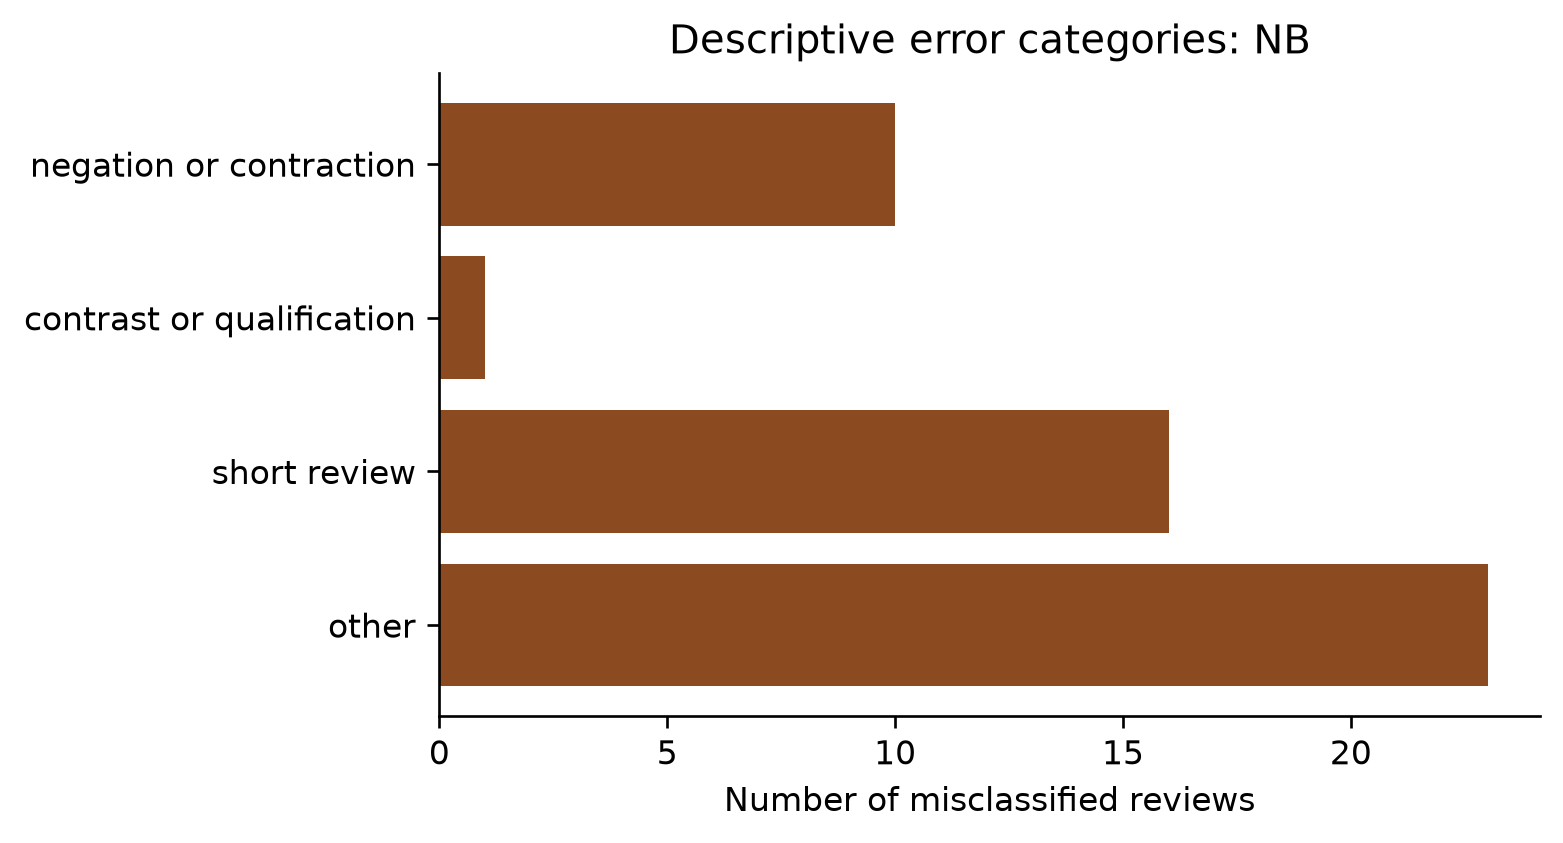
\includegraphics[width=\columnwidth]{../results/figures/final_error_categories.png}
  \caption{Primary descriptive error categories for the highest-F1 model on
  the test partition. Counts are produced by the fixed heuristic priority
  described above and are not causal labels.}
  \label{fig:error-categories}
\end{figure}

\section{Discussion}
\label{sec:discussion}

The experiment answers the three model questions in a limited but reproducible
way. Linear SVM did not outperform Multinomial NB on the fixed test sample: NB
was better in accuracy, recall, positive-class F1 and ROC-AUC, whereas SVM was
better in precision. Word unigrams were already selected by Member 3's
training-only comparison; bigrams did not improve the prespecified F1 and are
not re-tested here. The most discriminative terms are intuitive sentiment
words, but contraction handling and the absence of punctuation features
constrain interpretation.

Several limitations apply. The corpus contains 996 distinct short snippets,
so a 200-review test set gives imprecise estimates; small metric gaps should
not be treated as significant. The majority-class baseline reaches F1 0.667
only because it always predicts the positive class, which gives perfect recall
and no practical discrimination. Error categories rely on a small keyword
heuristic rather than human annotation, and the NB log-odds and SVM weights
are associations learned from this corpus. Finally, all reported numbers
use Member 4's locked $C=0.1$ SVM setting. Every table, figure and number in
this section is generated by
\texttt{restaurant\_sentiment.final\_evaluation} and recorded in
\texttt{results/tables/final\_evaluation.json}.


\section{Conclusion}

The experiment provides a reproducible comparison on this fixed small corpus.
Word bigrams increased dimensionality without improving the prespecified SVM
validation F1, so word unigrams were retained. Multinomial Naive Bayes achieved
the strongest held-out F1 and ROC--AUC, while the Linear SVM achieved higher
precision. The numerical gaps are modest and the test set contains only 200
reviews, so the result should be treated as evidence for this dataset rather
than a general ranking of the algorithms. Better contraction handling,
manually validated error labels, and a larger independently collected test set
would strengthen future work.

\section*{Impact Statement}

Sentiment classifiers can support aggregate service-quality analysis, but
their errors may misrepresent individual customers, dialects, sarcasm, or
mixed opinions. This study uses a small public educational dataset and does
not identify reviewers or restaurants. Predictions should not be used for
automated punitive decisions. We therefore report error patterns and model
limitations, keep raw text out of the repository, and frame feature weights as
correlations rather than causal explanations.

\bibliography{references}
\bibliographystyle{icml2026}

\end{document}
